\documentclass[10pt]{jarticle}
\usepackage{float}
\usepackage{adrobo_abst}
\usepackage[dvipdfmx]{graphicx}
\usepackage{amssymb,amsmath}
\usepackage{bm}
\usepackage[superscript]{cite}
\usepackage{enumerate}
\usepackage{url}
\usepackage{here}
%\usepackage[absolute]{textpos}

\renewcommand\citeform[1]{(#1)}

\begin{document}
    
    \makeatletter
    \doctype{2023年度卒業論文概要}
    \title{自律移動ロボットのためのYOLOv5を用いた\\AutoMSRCR画像からの水たまり検出}{}
    \etitle{Making Research Paper}{($\bigcirc\bigcirc\bigcirc$)}
    
    \author{20C1106\hspace{.5zw}松井大和}
    \eauthor{Yamato Matsui}
    
    \makeatother
    
    \abstract{When preparing the manuscript, read and observe carefully this sample as well as the instruction manual for the manuscript of the Transaction of Japan Society of Mechanical Engineers. This sample was prepared using MS-word. Character size of the English title is 14 pts of Times New Roman as well as sub-title. The name is 12 pts. The address of the first author and the abstract is 10 pts of Times New Roman. Character spacing of the abstract is narrowed by 0.2 pts preferably.}
    
    \keywords{Mechanical Engineering, Keywords List}
    
    \maketitle
    
    \supervisor{指導教員:上田隆一 准教授}
    
    \section{緒\hspace{2zw}言}%===========================
    
    近年, 日本では労働人口の減少が問題となっており, 
    その解決のため自律移動ロボットの利用が試みられている. 
    自律移動ロボットを施設の清掃や警備, 荷物の運搬などに利用するためには
    様々な技術が求められる. 
    特に障害物回避はロボットや環境の保護のために不可欠な技術であり, 
    これまで主に立体的な障害物を対象に研究開発が進められてきた. 
    しかしながら, 屋外には水たまりをはじめとする平面的な障害物も存在し, 
    それらの回避も求められる場合がある. ロボットが水たまり上を走行すると, 
    浸水による故障, 窪みによるスタックやオドメトリの誤差の増加, 
    水の飛散による周囲の人への被害などを及ぼすことが予測される. 
    したがって屋外自律移動ロボットには水たまりを検出し回避することが, 
    重要な課題となる.\\ 
     しかし, 水たまりは不規則な形状であることや景色の映り込みが発生しやすい性質から, 
    検出が困難である. そのため形状や反射光に左右されない検出手法が求められる.\\
      水たまり検出に関する取り組みとして, 
    色調を調整したカメラ画像からYOLOを用いて水たまり検出を行った研究がある. 
    Xiaodongら\cite{工大2005}はYOLOにおける通常のカメラ画像からの水たまり検出が困難である要因が水の性質による
    低コントラスト化にあると考え, 画像に処理をかけ水のコントラストを強化する手法を提案した. 
    この研究では複数の画像強化手法を比較検証し, 
    AutoMSRCR処理を施した画像を学習させたモデルで水たまりの検出性能の向上を確認している. 
    しかし, この研究では露出オーバーの発生した環境での有効性を確認したのみで, 
    自律移動ロボットが走行するような舗装された路面上や
    電信柱などの環境の映り込みが発生しやすい環境での有効性の確認がされていない.  
    また自律移動ロボットによる検出した水たまりの回避は行われていない. \\
     そこで, 本研究ではAutoMSRCR画像からの水たまり検出手法の移動ロボットを動かす環境への応用を目的とする. 
    具体的には舗装された路面上や映り込みが発生しやすい環境でのAutoMSRCR画像からの水たまり検出手法
    の有効性の検証と, 自律移動ロボットによる検出した水たまりの回避を行う.


    \section{手法}%===========================
        XiaodongらのAutoMSRCR画像からの水たまり検出手法と
        自律移動ロボットによる検出した水たまりの回避の手法について述べる. 
    \subsection{データセットの作成と学習}
     以下がXiaodongらの研究で用いたデータセットの作成と学習の手順である. 
    \begin{quote}
        \begin{itemize}
         \item 水たまりを含む画像の撮影
         \item 撮影した画像にAutoMSRCR処理
         \item 水たまり部分をアノテーション
         \item YOLOを用いて学習
        \end{itemize}
       \end{quote}
    自律移動ロボットが走行するような環境での本手法の有効性の検証が目的となるため
    映り込みの多い環境や舗装された路面の水たまりを中心に撮影する. 今回は651枚の画像を用意した. 
    撮影した画像に対しAutoMSRCR処理を適用する. 
    \begin{figure}[H]
        \begin{tabular}{cc}
            \begin{minipage}{.1\textwidth}
                \vspace{5mm}\centering
                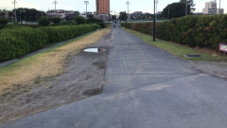
\includegraphics[width=2.0\linewidth]{./fig/fig1.png}
                \caption{Original}
                \label{fig_first}
            \end{minipage}
            \begin{minipage}{.5\textwidth}
                \vspace{5mm}\centering\centering
                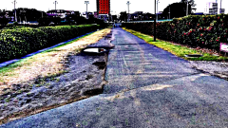
\includegraphics[width=0.4\linewidth]{./fig/fig2.png}
                \caption{AutoMSRCR}
                \label{fig_second}
            \end{minipage}
        \end{tabular}
    \end{figure}
    その際データセットの作成に使用する画像と推定に用いる画像の両方に適用する. 
    アノテーションツールにはVoTTを使用し, 1クラスのみでタグ付けを行う. 
    このようにして作成したデータセットをYOLOv5を用いて学習する. 

    \subsection{検出した水たまりの回避}
    (実装が間に合っていないため終わりしだい追記予定)

    \section{実験}%===========================
    舗装された路面上や映り込みが発生しやすい環境でのAutoMSRCR画像からの水たまり検出手法
    の有効性を検証する. 
    \subsection{移動ロボットを動かす環境でのAutoMSRCR画像からの水たまり検出手法の有効性の検証}
     評価のため用意した水たまりを含む画像から10枚を抽出し, 
    オリジナル画像の学習モデルとAutoMSRCR画像の学習モデルのそれぞれを使用して推定, 評価を行う. \\
     評価基準は以下のものとする. 
    \begin{quote}
        \begin{itemize}
         \item Recall(R) 
         \item Precision(P) 
         \item しきい値: IoU 0.5
         \item RとP両方の値が1.0だった場合を正解とする
         
        \end{itemize}
       \end{quote}
     検証の結果, オリジナル画像の学習モデル(表1)は検出率が4/10であったのに対し, 
    AutoMSRCR画像の学習モデル(表2)では検出率が6/10まで向上した. 
    このことから舗装された路面上や映り込みが発生しやすい環境においてもこの手法は有効であると言える. 

    \begin{center}
        \begin{figure}[H]
            \caption{Sample}
            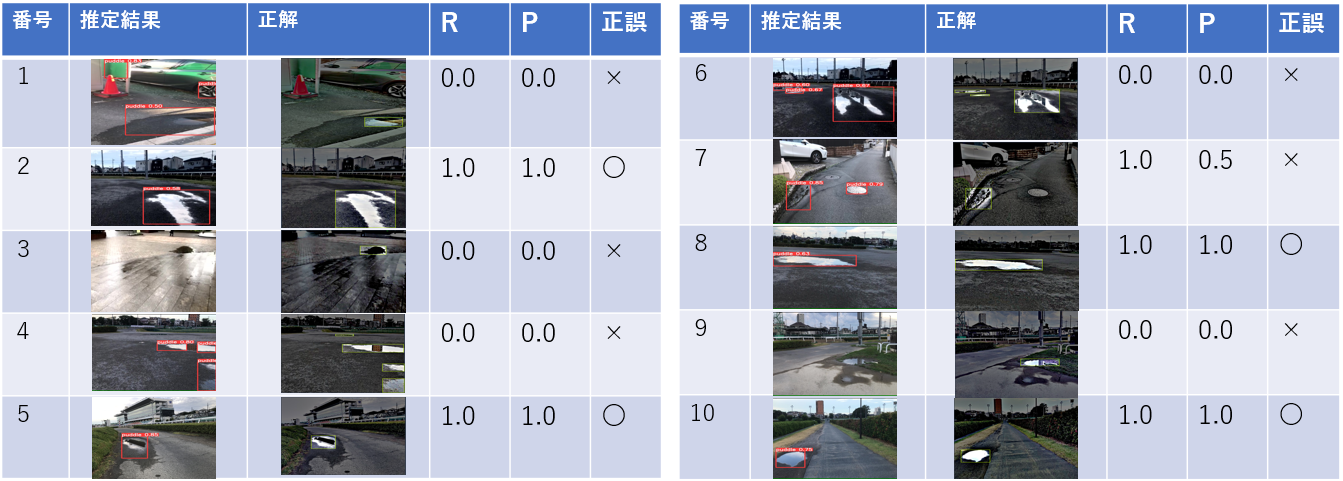
\includegraphics[width=0.45\textwidth]{./fig/fig3.png}
            \label{fig:sample-fig}
        \end{figure}
    \end{center}
    \begin{center}
        \begin{figure}[H]
            \caption{Sample}
            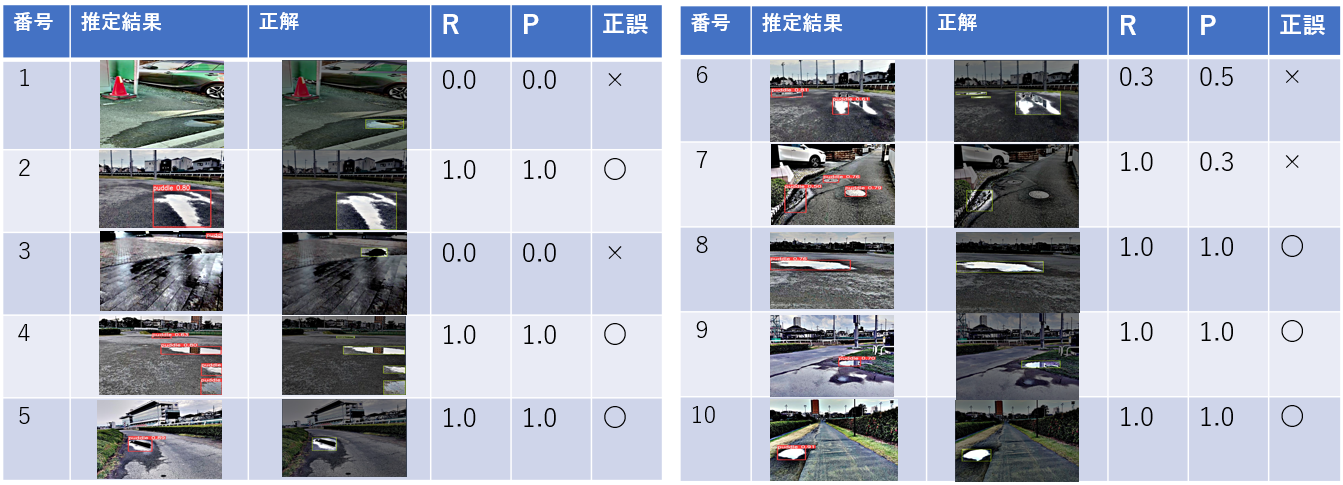
\includegraphics[width=0.45\textwidth]{./fig/fig4.png}
            \label{fig:sample-fig}
        \end{figure}
    \end{center}

    \subsection{検出した水たまりの回避}
    (実装が間に合っていないため終わりしだい追記予定)

    \section{結言}%===========================



    



    
    
 
    \vspace{5truemm}
    {\footnotesize
        \begin{thebibliography}{99}
            
            \bibitem{工大2005}
            工大太郎: ``ロボットのしくみ'', 
            日本機械学会論文誌A, 
            Vol.~108, No.~1034 (2005), pp.~1--2.
            
            \bibitem{Shibutani2004}
            Y. Shibutani: ``Heinrich's Law Resulted Pattern Dynamics --Part2--'',
            Proceedings of the 79th Kansai Branch Regular Meeting of the Japan Society of Mechanical Engineers,  
            No.~04--05 (2004), pp.~205--206.
            
            \bibitem{Handbook1979}
            The Japan Society of Mechanical Engineers ed.: ``JSME Date Handbook: Heat Transfer'', 
            (1979), p.~123, The Japan Society of Mechanical Engineers.
            
            \bibitem{Kikuchi2017}
            K. Kikuchi, M. Miura, K. Shibata, J. Yamamura: ``Soft Landing Condition for Stair-climbing Robot with Hopping Mechanism'', 
            Journal of JSDE, Vol.~53, No.~8 (2018), pp.~605--614, \url{https://doi.org/10.14953/jjsde.2017.2774}.
            
            \bibitem{Adrobo2019}
            千葉工業大学 未来ロボティクス学科 学科概要: 
            \url{http://www.robotics.it-chiba.ac.jp/ja/subject/index.html}, 
            (参照日 2023年1月29日). 
            
        \end{thebibliography}
    }
    \normalsize
    
\end{document}
